\documentclass[14pt,a4paper]{extarticle}

\usepackage[T2A]{fontenc}
\usepackage[utf8]{inputenc}
\usepackage[ukrainian]{babel}
\usepackage{geometry}
\usepackage{setspace}
\usepackage{indentfirst}
\usepackage{amsmath}
\usepackage{amssymb}
\usepackage{graphicx}
\usepackage{float}
\usepackage{xcolor}
\usepackage{listings}
\usepackage{hyperref}

\geometry{left=25mm,right=15mm,top=20mm,bottom=20mm}
\onehalfspacing

\hypersetup{
    colorlinks=true,
    linkcolor=black,
    urlcolor=blue,
    citecolor=black
}

\lstdefinelanguage{Maple}{
  morekeywords={restart,with,plot,plot3d,animate,piecewise,diff,Diff,int,Int,solve,fsolve,dsolve,pdsolve,series,evalf,collect,coeff,factor,expand,normal,convert,seq,array,matrix,det,matadd,allvalues,unapply},
  sensitive=true,
  morecomment=[l]{\#},
  morestring=[b]"
}

\lstset{
  language=Maple,
  basicstyle=\ttfamily\small,
  keywordstyle=\color{blue!70!black}\bfseries,
  commentstyle=\color{green!40!black},
  stringstyle=\color{red!60!black},
  frame=single,
  breaklines=true,
  keepspaces=true,
  tabsize=2,
  showstringspaces=false
}

\begin{document}

\begin{titlepage}
    \centering
    {\small Міністерство освіти і науки України\par}
    {\small \textbf{Київський національний університет імені Тараса Шевченка}\par}
    {\small Факультет комп'ютерних наук та кібернетики\par}
    \vspace{18mm}

    {\large\bfseries ЗВІТ\par}
    {\large до лабораторної роботи №1\par}
    \vspace{2mm}
    {\large з дисципліни «Комп'ютерне моделювання»\par}
    \vspace{8mm}

    {\Large\bfseries Тема: Базові можливості Maple\par}

    \vfill

    \begin{flushright}
        Виконав: студент 1 курсу магістратури\\
        групи ПМ\\
        Кіщук Ярослав Ярославович
    \end{flushright}

    \vfill
    {\small Київ --- 2026\par}
\end{titlepage}

\section*{Назва роботи}
Лабораторна робота №1 «Базові можливості системи Maple для математичного моделювання».

\section*{Мета роботи}
Ознайомитися з базовими засобами Maple для:
\begin{itemize}
    \item виконання аналітичних обчислень;
    \item роботи з виразами та структурами даних;
    \item побудови двовимірної й тривимірної графіки;
    \item аналітичного та чисельного розв'язання рівнянь і диференціальних рівнянь.
\end{itemize}

\section*{Лістинги виконаних завдань з функціями}

\subsection*{1. Табл. 1.21--1.24}
\begin{lstlisting}
restart;
S := seq(i, i=1..10);
P := {seq(a[i], i=1..5)};
L := [sin, cos, tan];
A := array(1..5);
\end{lstlisting}

\textbf{Результат:} Виконання команд у Maple дало такі результати:
\begin{itemize}
    \item \texttt{S := 1, 2, 3, 4, 5, 6, 7, 8, 9, 10} --- послідовність типу \texttt{exprseq} з 10 елементів, сформована оператором \texttt{seq}.
    \item \texttt{P := \{a[1], a[2], a[3], a[4], a[5]\}} --- множина типу \texttt{set} з 5 іменованих елементів.
    \item \texttt{L := [sin, cos, tan]} --- список типу \texttt{list}.
    \item \texttt{A := array(1..5, [])} --- порожній масив типу \texttt{array} з індексами від 1 до 5.
\end{itemize}

\begin{figure}[H]
    \centering
    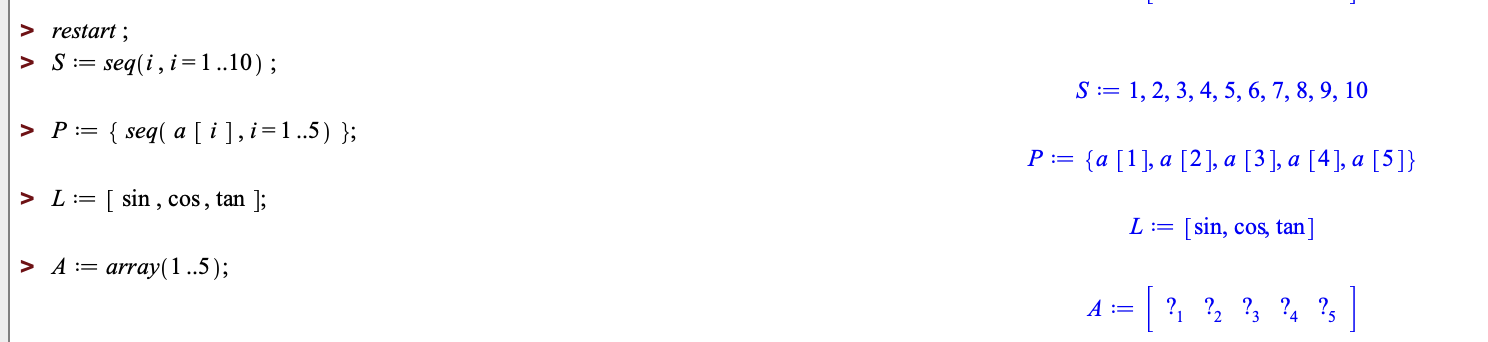
\includegraphics[width=\textwidth]{listing1_result}
    \caption{Результати виконання лістингу 1 у Maple}
\end{figure}

\subsection*{2. Операції з формулами (табл. 1.25--1.29)}
\begin{lstlisting}
expr1 := sin(x)^2 + cos(x)^2;
simplify(expr1);

expr2 := (x+1)*(x+2);
expand(expr2);

p := 2*x^2 + 3*y^3 - 5;
coeff(p, x, 0);
\end{lstlisting}
\textbf{Результат:} Виконання команд у Maple дало такі результати:
\begin{itemize}
    \item для \texttt{expr1 := sin(x)\^{}2 + cos(x)\^{}2} після \texttt{simplify(expr1)} отримано \texttt{1};
    \item для \texttt{expr2 := (x+1)*(x+2)} після \texttt{expand(expr2)} отримано \texttt{x\^{}2 + 3*x + 2};
    \item для \texttt{p := 2*x\^{}2 + 3*y\^{}3 - 5} команда \texttt{coeff(p, x, 0)} повертає \texttt{3*y\^{}3 - 5}.
\end{itemize}

\begin{figure}[H]
    \centering
    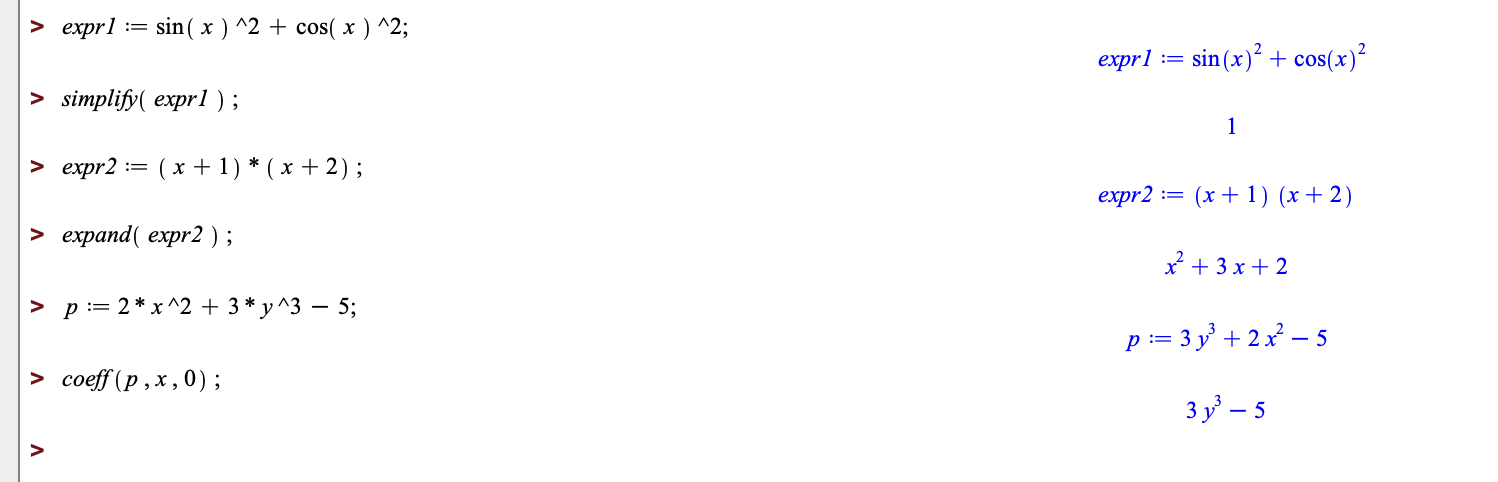
\includegraphics[width=\textwidth]{listing2_result}
    \caption{Результати виконання лістингу 2 у Maple}
\end{figure}

\subsection*{3. Похідні та інтеграли (табл. 1.30--1.35)}
\begin{lstlisting}
diff(sin(x), x$2);
Int(sin(x), x=0..Pi/4) = int(sin(x), x=0..Pi/4);
evalf(Int(sin(x), x=0..Pi/4));
\end{lstlisting}
\textbf{Результат:} Виконання команд у Maple дало такі результати:
\begin{itemize}
    \item \texttt{diff(sin(x), x\$2)} $\rightarrow$ \texttt{-sin(x)};
    \item \texttt{Int(sin(x), x=0..Pi/4) = int(sin(x), x=0..Pi/4)} $\rightarrow$ \texttt{\(\int_0^{\pi/4} \sin(x)\,dx = 1 - \sqrt{2}/2\)};
    \item \texttt{evalf(Int(sin(x), x=0..Pi/4))} $\rightarrow$ \texttt{0.2928932188}.
\end{itemize}

\begin{figure}[H]
    \centering
    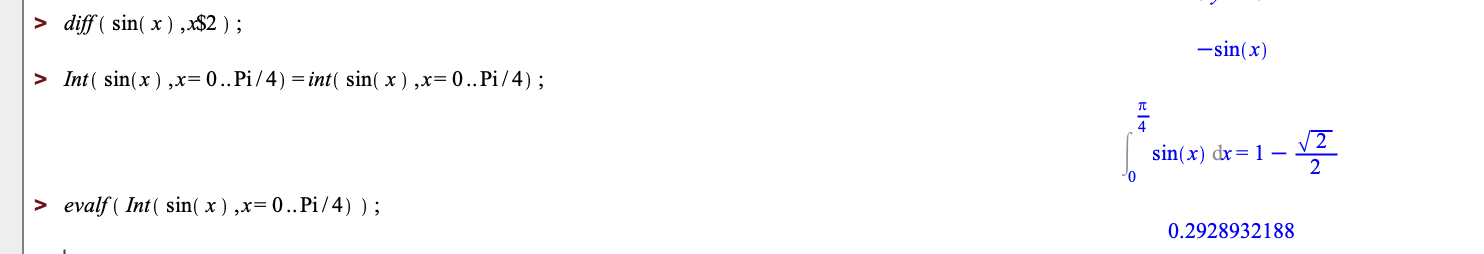
\includegraphics[width=\textwidth]{listing3_result}
    \caption{Результати виконання лістингу 3 у Maple}
\end{figure}

\subsection*{4. Пакети, 2D-графіка та анімація (табл. 1.36--1.39)}
\begin{lstlisting}
with(linalg):
A := matrix(3,3,[[1,2,3],[4,5,6],[7,8,9]]);
B := matrix(3,3,[[7,4,3],[1,2,5],[8,9,6]]);
det(A); det(B); matadd(A,B);

plot(sin(x), x=0..2*Pi, style=POINT);
with(plots):
animate(sin(x*t), x=-10..10, t=1..2);
\end{lstlisting}
\textbf{Результат:} Виконання команд у Maple дало такі результати:
\begin{itemize}
    \item після підключення \texttt{with(linalg)} обчислено визначники матриць: \texttt{det(A)=0}, \texttt{det(B)=-116};
    \item знайдено суму матриць: \texttt{matadd(A,B) = [[8,6,6],[5,7,11],[15,17,15]]};
    \item побудовано 2D-графік \texttt{plot(sin(x), x=0..2*Pi, style=POINT)} у точковому стилі;
    \item створено анімацію \texttt{animate(sin(x*t), x=-10..10, t=1..2)}.
\end{itemize}

\begin{figure}[H]
    \centering
    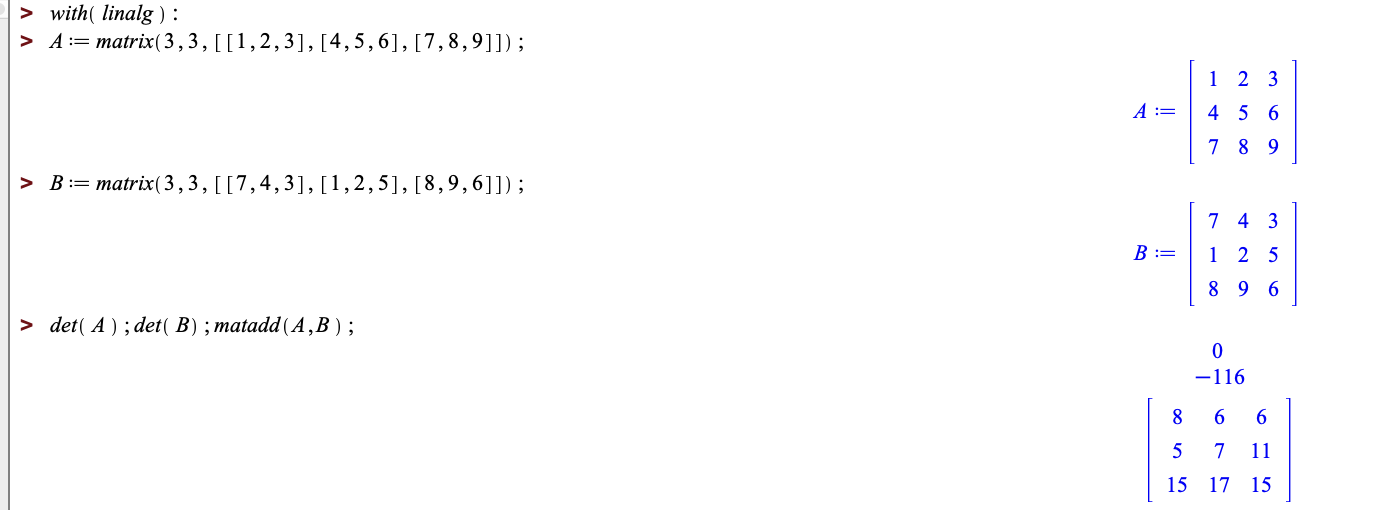
\includegraphics[width=\textwidth]{listing4_result_1}
    \caption{Результати обчислень пакета \texttt{linalg} (лістинг 4, скріншот 1)}
\end{figure}

\begin{figure}[H]
    \centering
    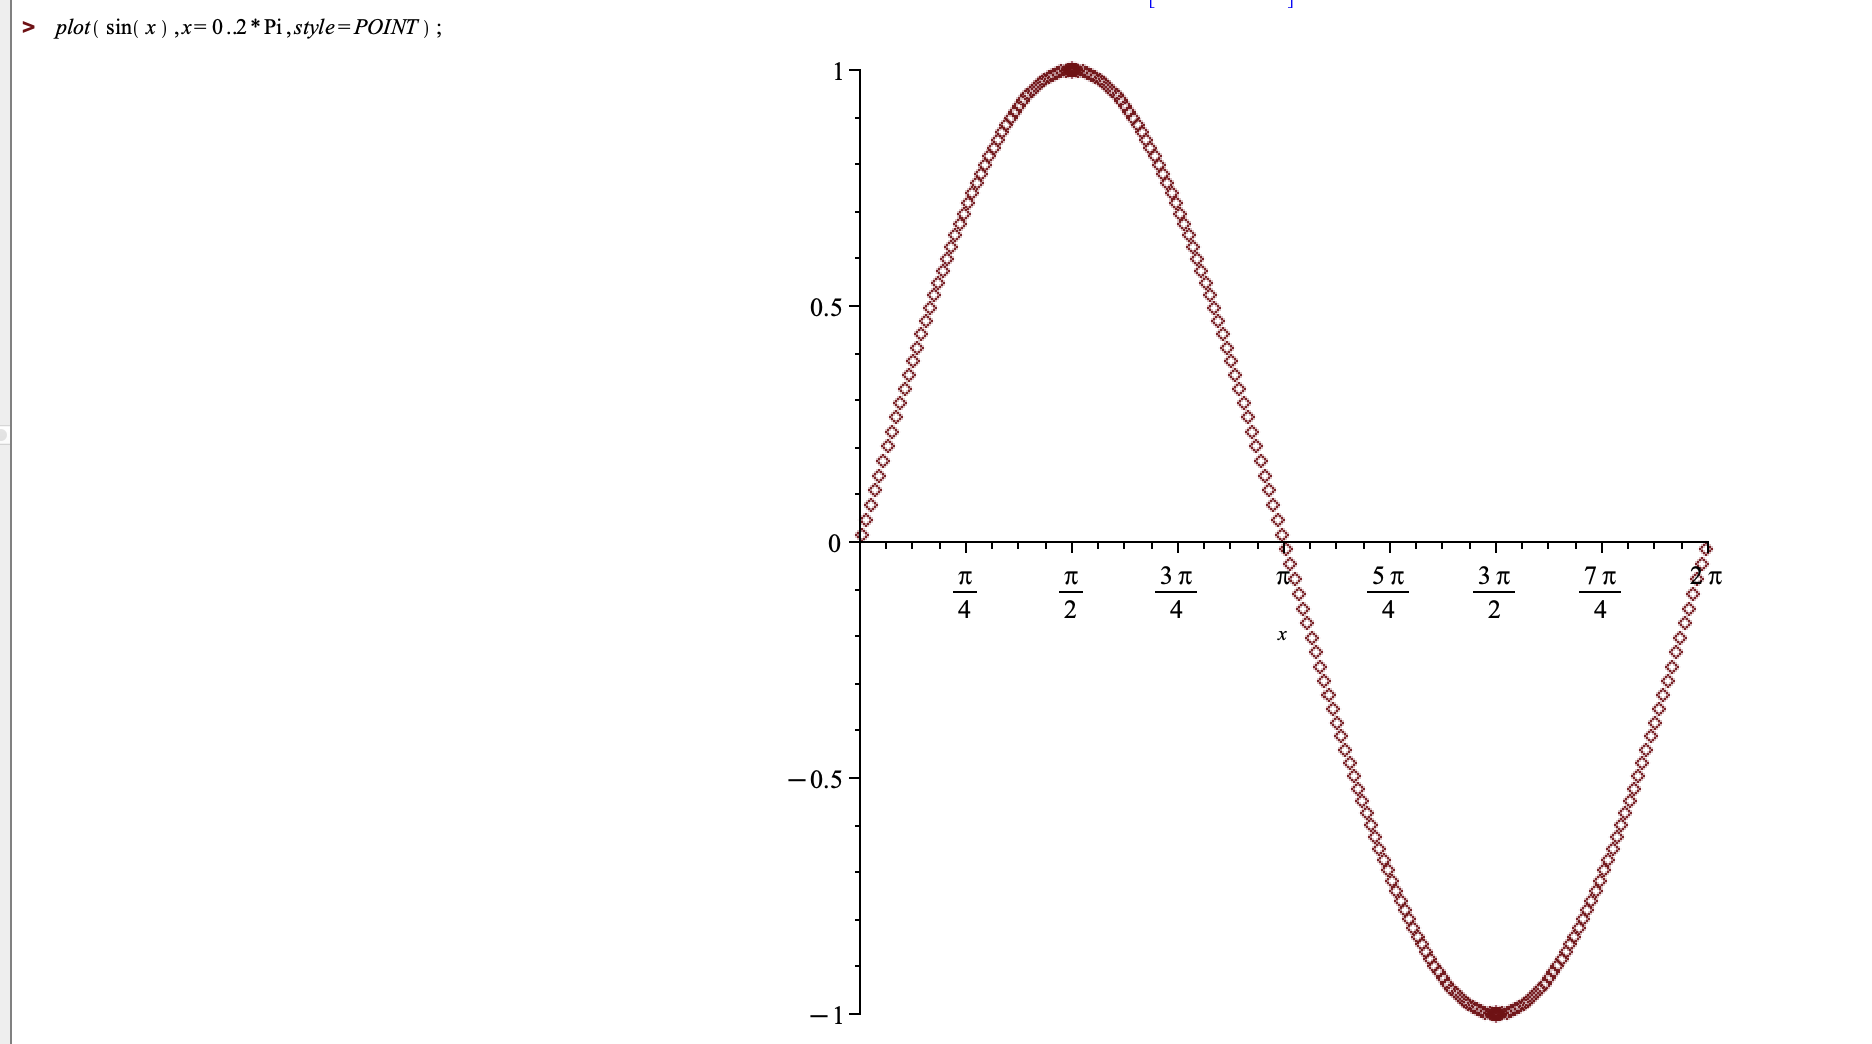
\includegraphics[width=\textwidth]{listing4_result_2}
    \caption{Побудова графіка \texttt{sin(x)} у стилі \texttt{POINT} (лістинг 4, скріншот 2)}
\end{figure}

\begin{figure}[H]
    \centering
    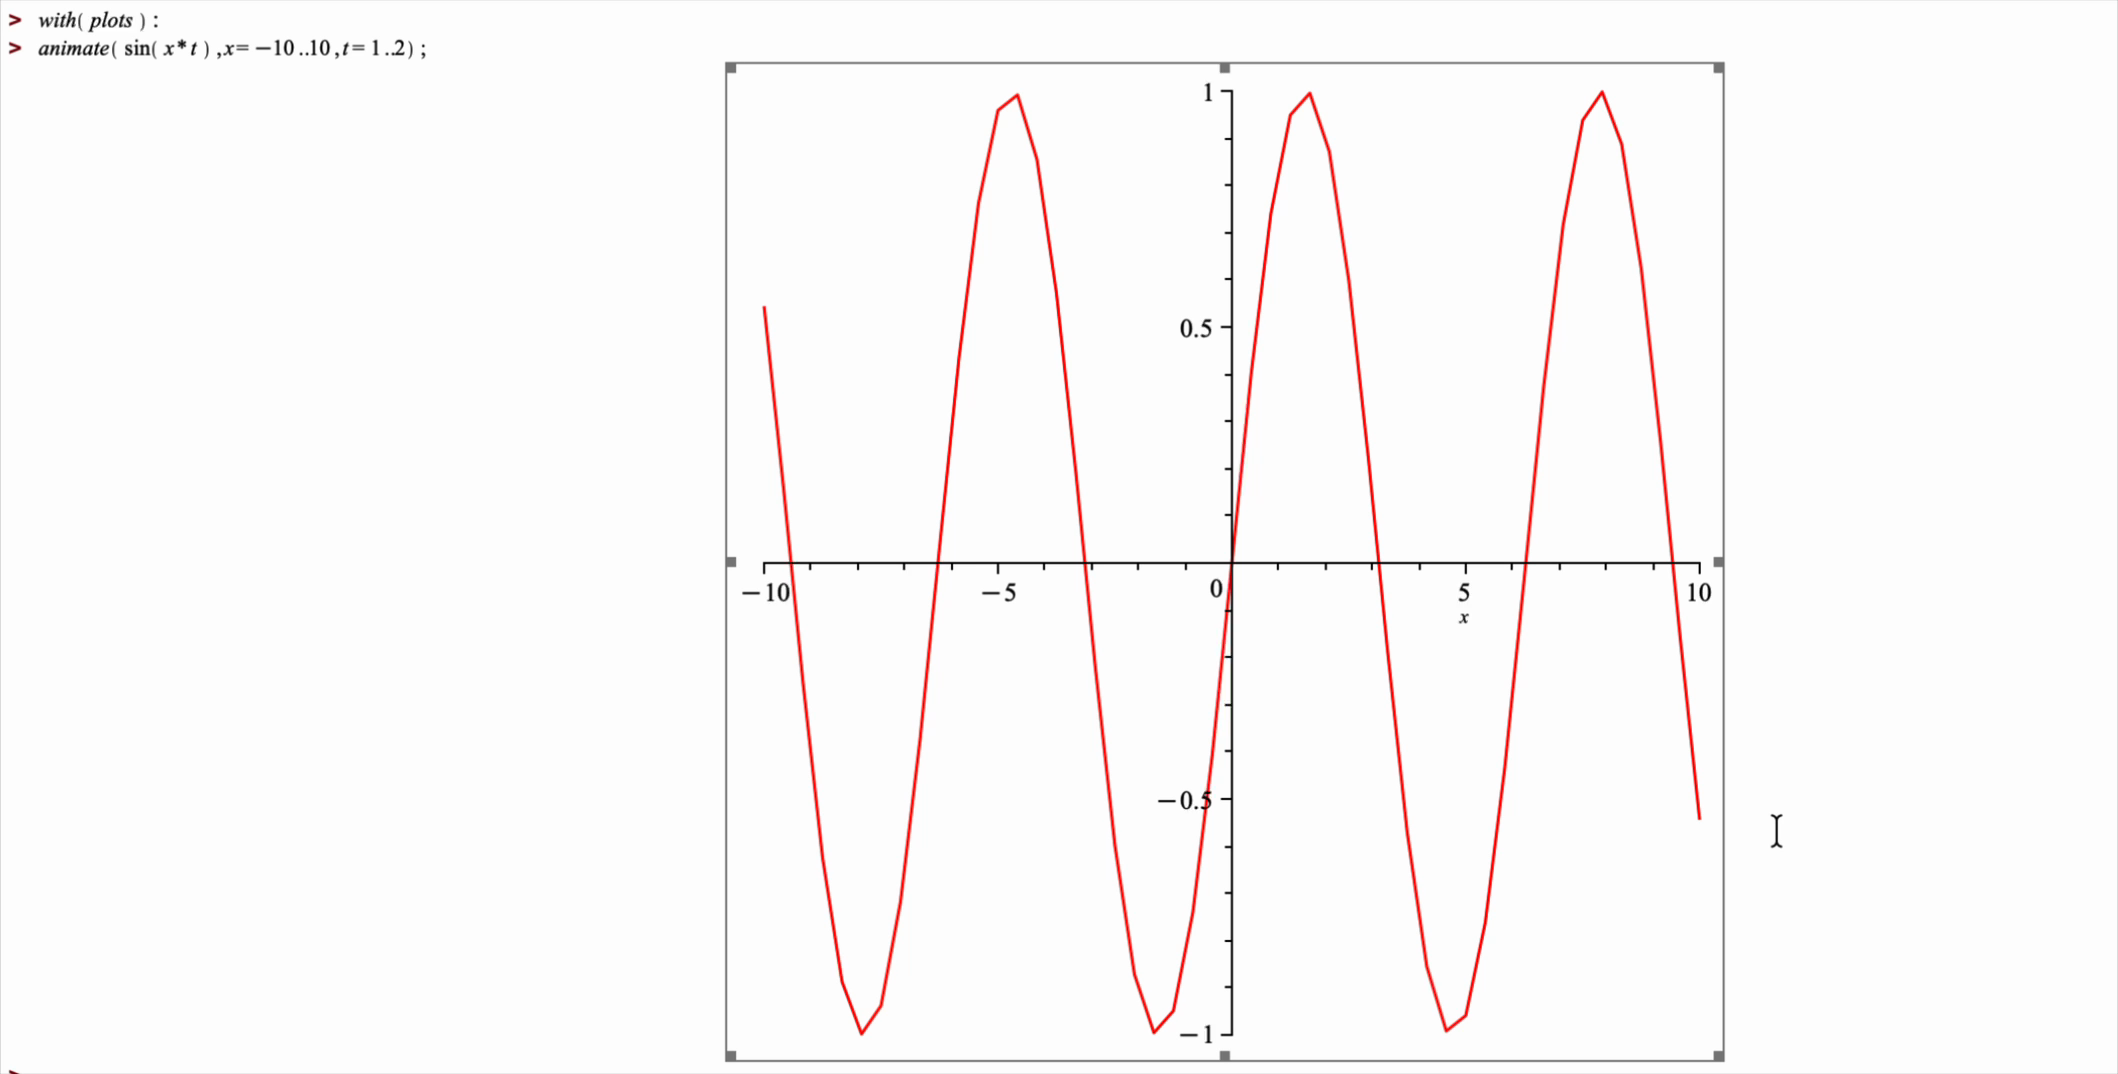
\includegraphics[width=\textwidth]{listing4_animation_preview}
    \caption{Кадр анімації для лістингу 4 (GIF: \texttt{listing4\_animation.gif})}
\end{figure}

\subsection*{5. Кусково-задані функції та 3D-графіка (табл. 1.40--1.41)}
\begin{lstlisting}
p := x -> piecewise(x<0, -x, x>0, x);
plot(p(x), x=-1..1, scaling=constrained);

plot3d(x*exp(-x^2-y^2), x=-2..2, y=-2..2, grid=[25,25]);
\end{lstlisting}
\textbf{Результат:} Виконання команд у Maple дало такі результати:
\begin{itemize}
    \item задано кусково-неперервну функцію \texttt{p := x -> piecewise(x<0, -x, x>0, x)};
    \item побудовано її графік на проміжку \texttt{x=-1..1} з параметром \texttt{scaling=constrained};
    \item побудовано тривимірний графік функції \texttt{x*exp(-x\^{}2-y\^{}2)} на області \texttt{x=-2..2}, \texttt{y=-2..2} з сіткою \texttt{grid=[25,25]}.
\end{itemize}

\begin{figure}[H]
    \centering
    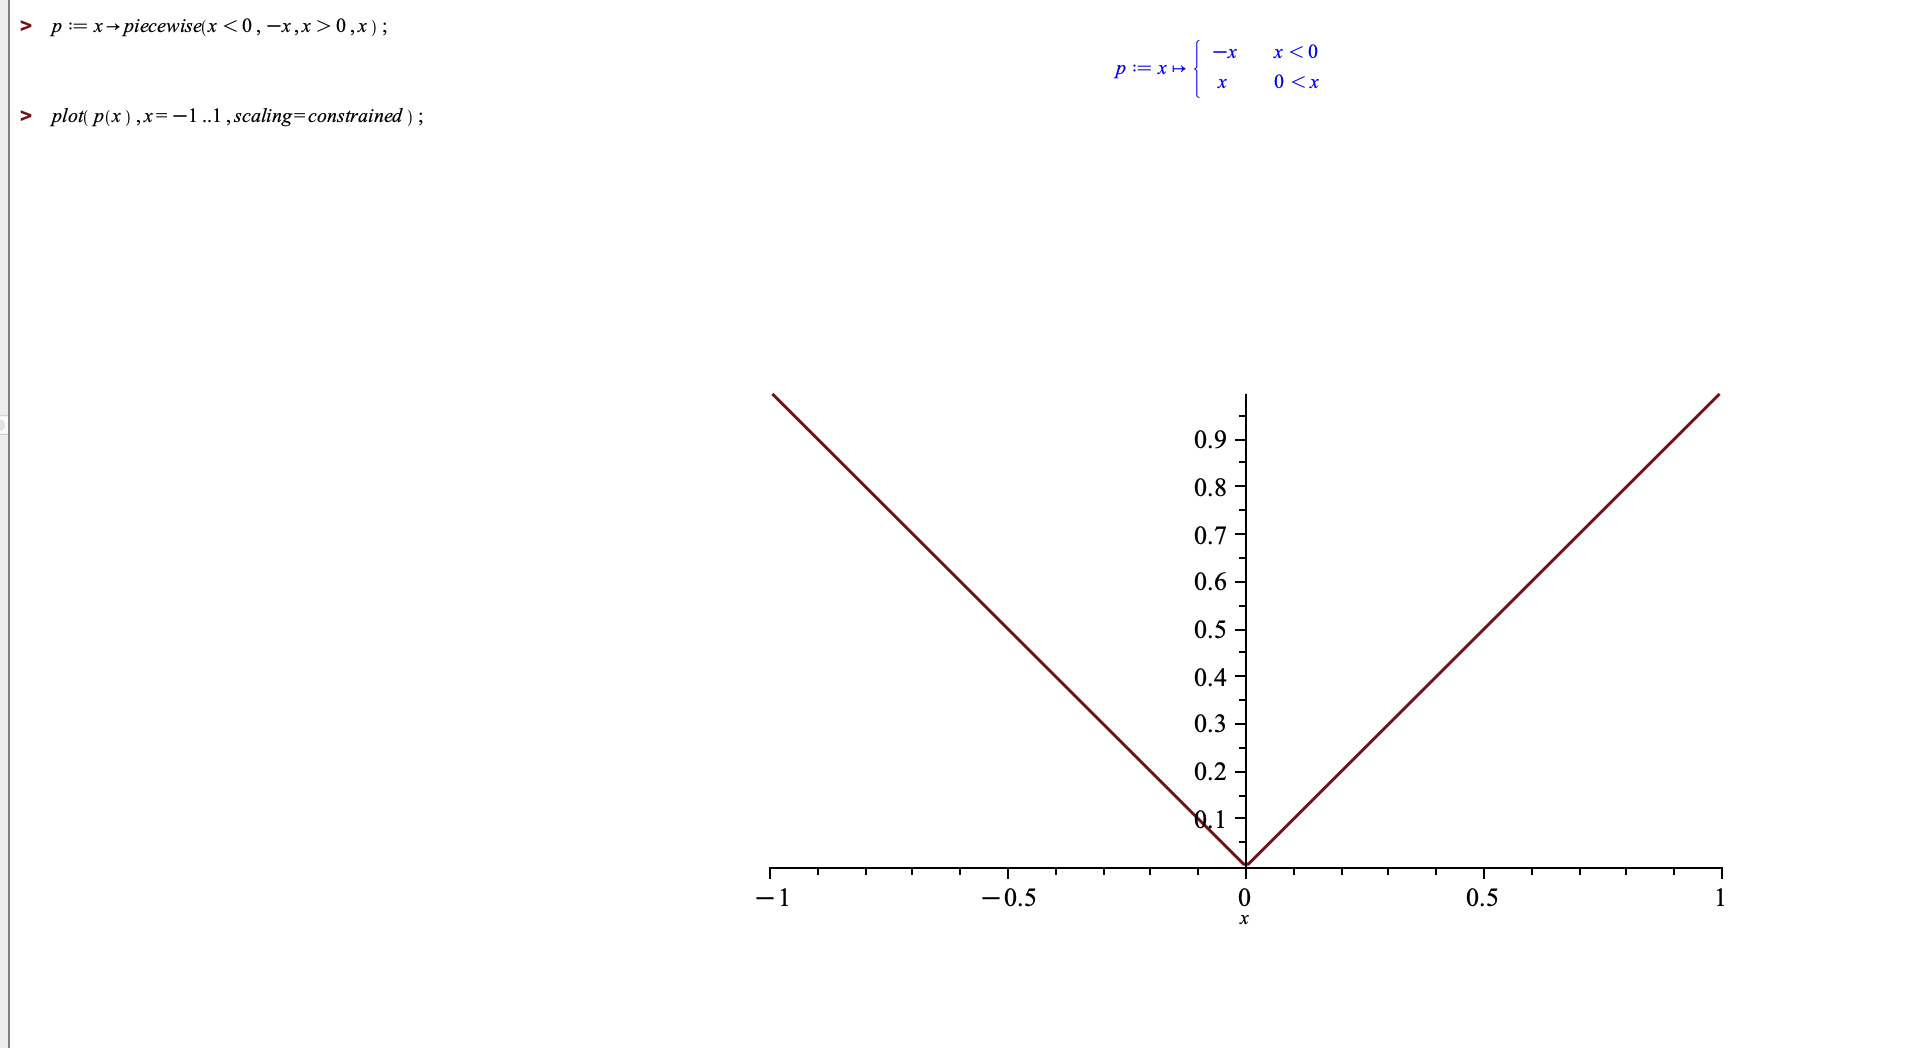
\includegraphics[width=\textwidth]{listing5_result_1}
    \caption{Побудова кусково-заданої функції у Maple (лістинг 5, скріншот 1)}
\end{figure}

\begin{figure}[H]
    \centering
    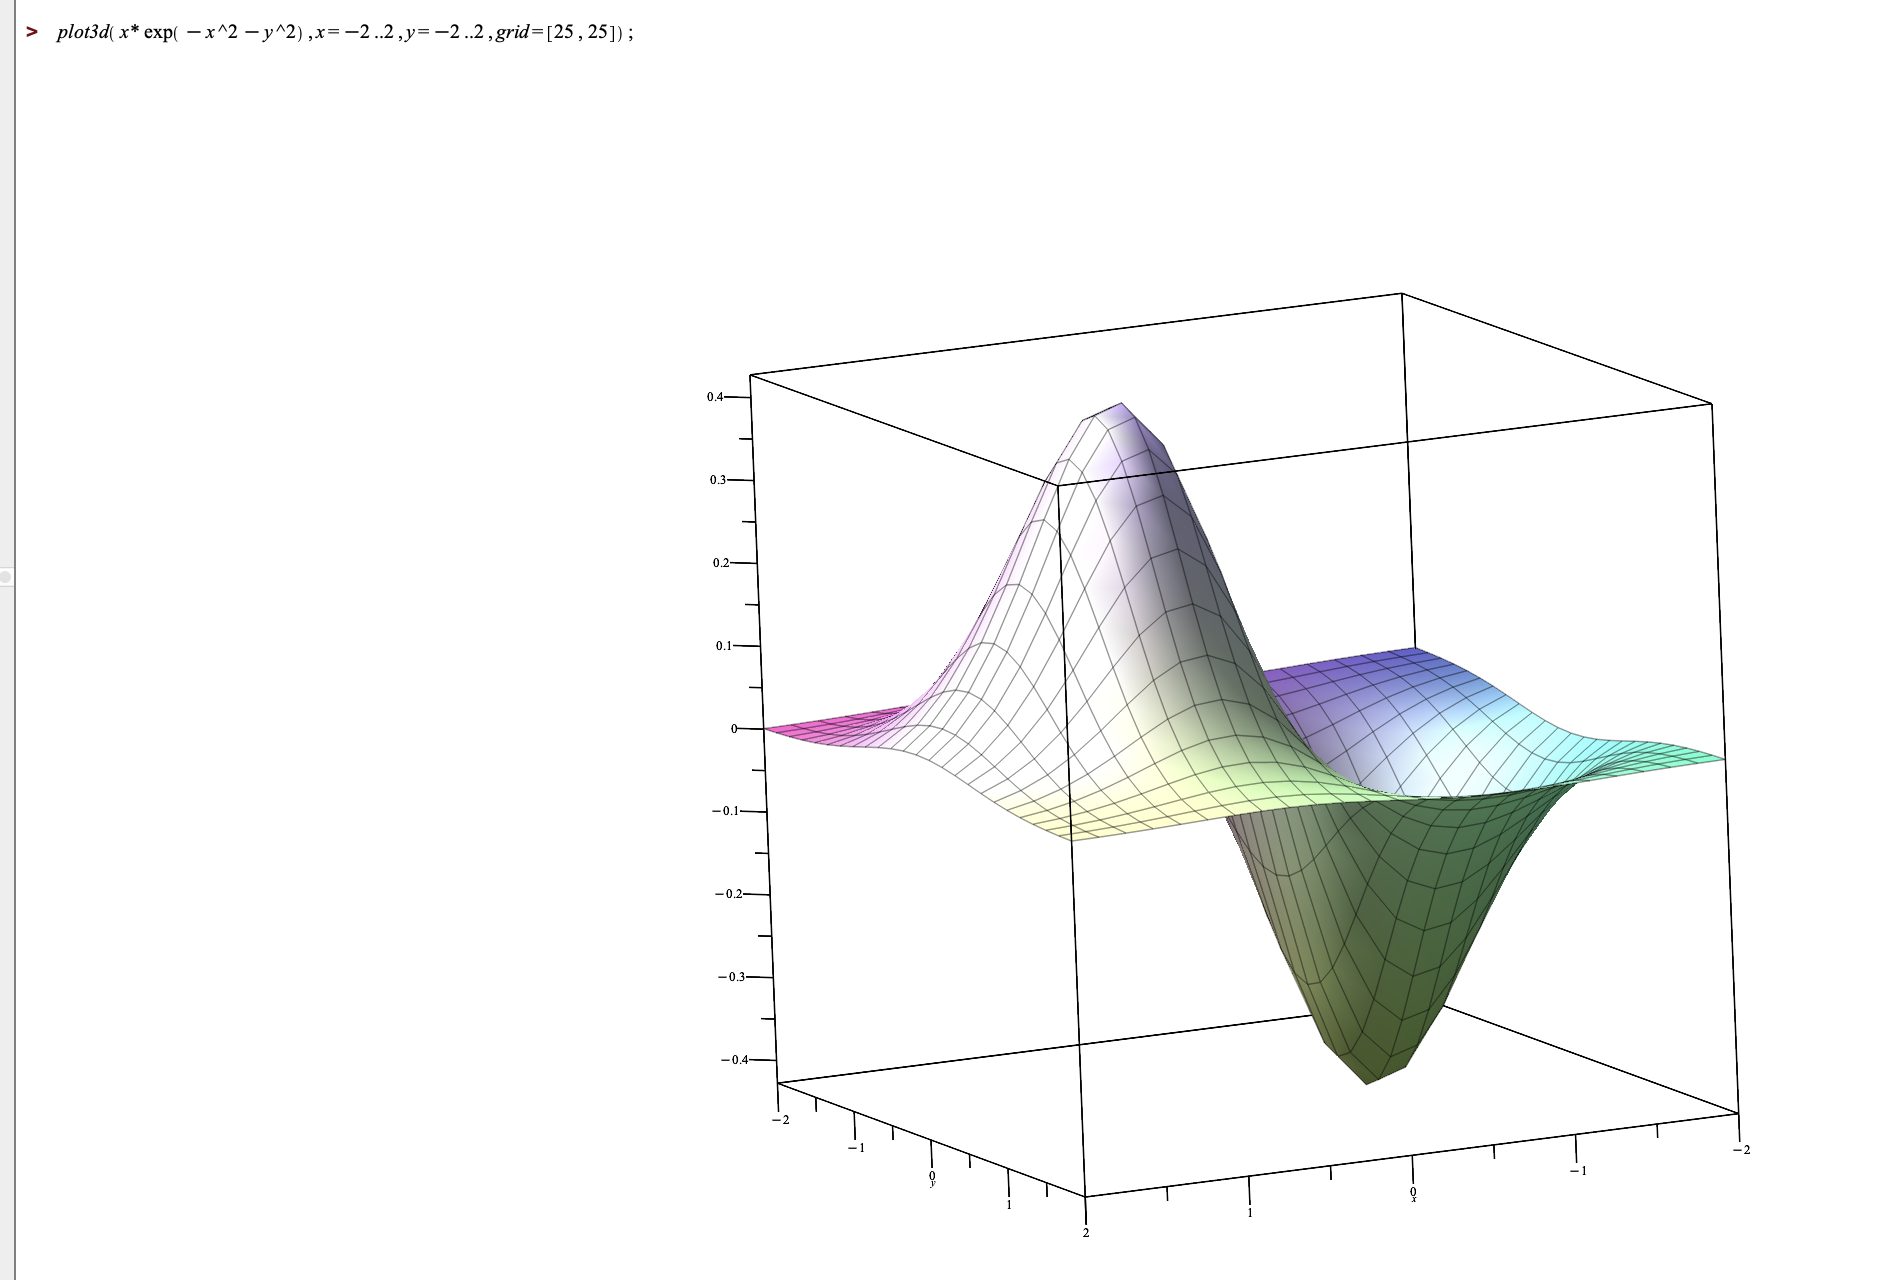
\includegraphics[width=\textwidth]{listing5_result_2}
    \caption{Побудова тривимірного графіка у Maple (лістинг 5, скріншот 2)}
\end{figure}

\subsection*{6. Рівняння та системи (табл. 1.42--1.44)}
\begin{lstlisting}
solve(a*x^2+b*x+c=0, x);
solve({x+5*y+z=1, 2*x-y+4*z=4, x+2*y+2*z=12}, {x,y,z});
fsolve(cos(x)-(x+2)/(x-2), x=-6..-4);
\end{lstlisting}
\textbf{Результат:} Виконання команд у Maple дало такі результати:
\begin{itemize}
    \item для рівняння \texttt{a*x\^{}2+b*x+c=0} отримано загальний розв'язок за формулою квадратного рівняння: \texttt{x = (-b \textbackslash{}pm sqrt(b\^{}2-4*a*c))/(2*a)};
    \item для системи \texttt{\{x+5*y+z=1, 2*x-y+4*z=4, x+2*y+2*z=12\}} отримано розв'язок \texttt{\{x=-42, y=4, z=23\}};
    \item чисельний розв'язок рівняння \texttt{cos(x)-(x+2)/(x-2)=0} на проміжку \texttt{x=-6..-4} дорівнює \texttt{-5.170382990}.
\end{itemize}

\begin{figure}[H]
    \centering
    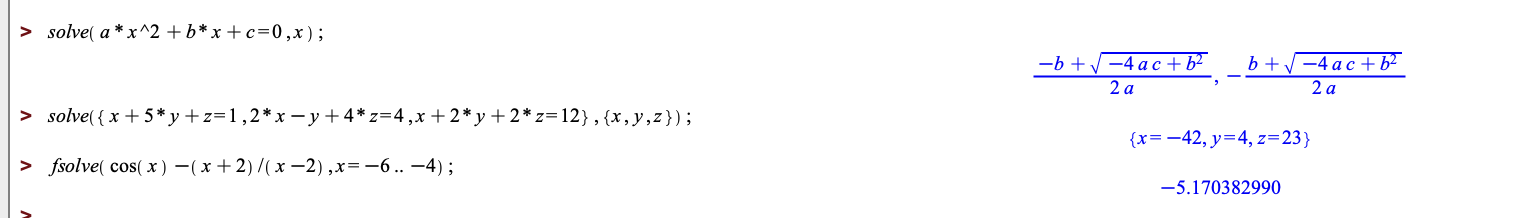
\includegraphics[width=\textwidth]{listing6_result}
    \caption{Результати виконання лістингу 6 у Maple}
\end{figure}

\subsection*{7. Звичайні диференціальні рівняння та їх системи (табл. 1.45--1.47)}
\begin{lstlisting}
ode := diff(y(x),x)/(2*x) + 3*x*y(x) = exp(-2*x^3);
R1 := dsolve({ode, y(0)=5});
R3 := dsolve({ode, y(0)=5}, numeric);

SYS := {diff(x(t),t)=y(t)-x(t), diff(y(t),t)=-x(t)-3*y(t), x(1)=0, y(1)=1};
dsolve(SYS, {x(t), y(t)});
\end{lstlisting}
\textbf{Результат:}
Аналітичний розв'язок диференціального рівняння першого порядку:
\[
R_1 = y(x) = (x^2 + 5)\,e^{-2x^3}
\]
Числовий розв'язок отримано методом RKF45:
\begin{lstlisting}
R3 := proc(x_rkf45) ... end proc
\end{lstlisting}
Для системи диференціальних рівнянь \texttt{dsolve(SYS, \{x(t), y(t)\})} повертає
аналітичний розв'язок через узагальнені власні вектори (подвійне власне
значення $\lambda = -2$).

\begin{figure}[H]
  \centering
  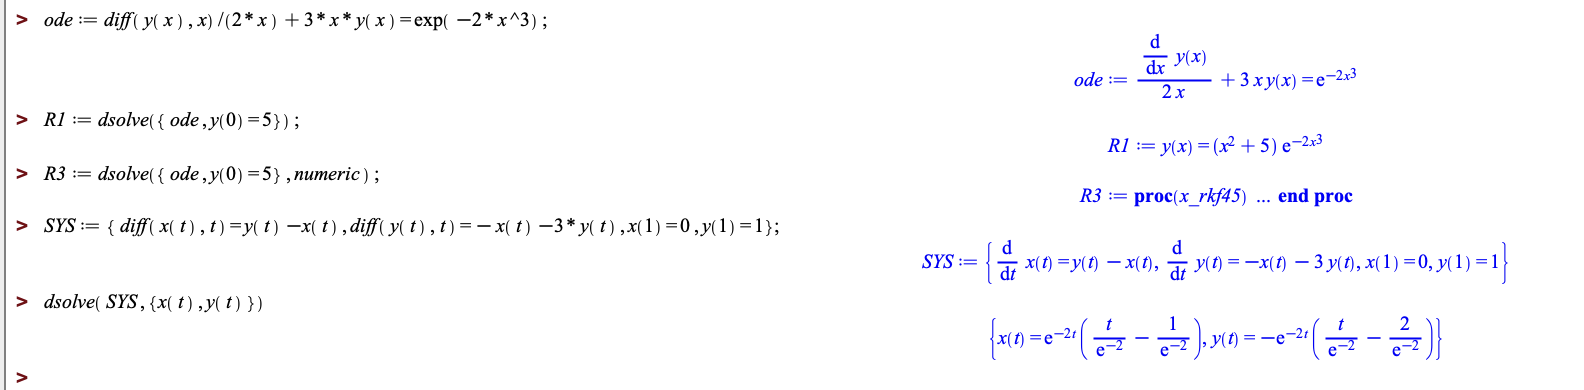
\includegraphics[width=0.9\linewidth]{listing7_result.png}
    \caption{Результати лістингу 7: диференціальне рівняння та система диференціальних рівнянь}
\end{figure}

\section*{Висновки}
У лабораторній роботі опановано базові інструменти Maple для аналітичних і
чисельних обчислень, перетворення математичних виразів, побудови 2D/3D графіків,
розв'язання алгебраїчних рівнянь, систем та диференціальних рівнянь. Отримані
навички дозволяють застосовувати Maple для задач математичного моделювання
фізичних і біологічних процесів.

\end{document}